\documentclass[a4paper]{article}
\usepackage[top=1in, bottom=1.25in, left=1.25in, right=1.25in]{geometry}


\usepackage{amsmath}
\usepackage{amssymb}
\usepackage{graphicx}
\usepackage[utf8]{inputenc}
 
\usepackage{amsthm}
\usepackage{enumitem}   
\usepackage{listings}

\lstset{
  breaklines=true,
  numbers=left,
  language=Python
}

\begin{document}

%% Title, authors and addresses

\title{Brain Inspired Computing - Problem Set 1}

\author{Sven Bordukat, Paul Meehan}

\date{\today}

\maketitle

\section*{Exercise 1}
As there are approximately $10^{11}$ neurons in the brain, each firing at around
1 Hz, and the total energy use is 20 W, we calculate the energy use per neuron:
\begin{align}
    E_{spike} &= \frac{20 J/s}{10^{11}*1/s}\\
    &= 2 * 10^{-10} J
\end{align}

\section*{Exercise 2}
\begin{itemize}
    \item[a)] 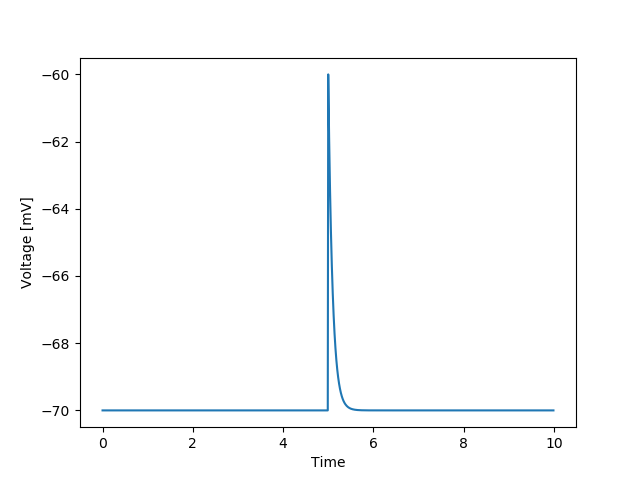
\includegraphics{a.png}
    \item[b)] 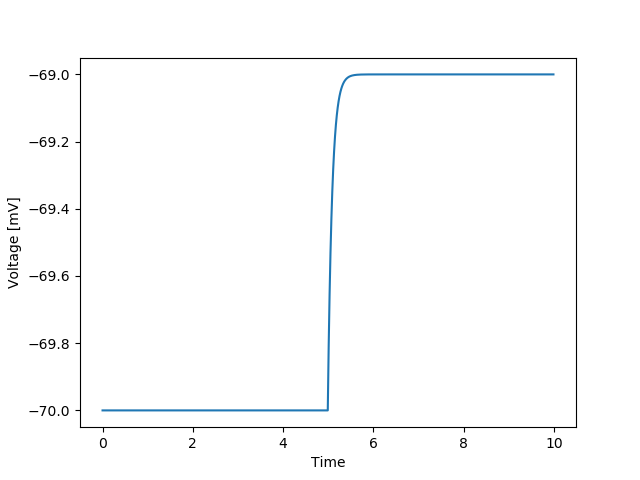
\includegraphics{b.png}
    \item[c)] 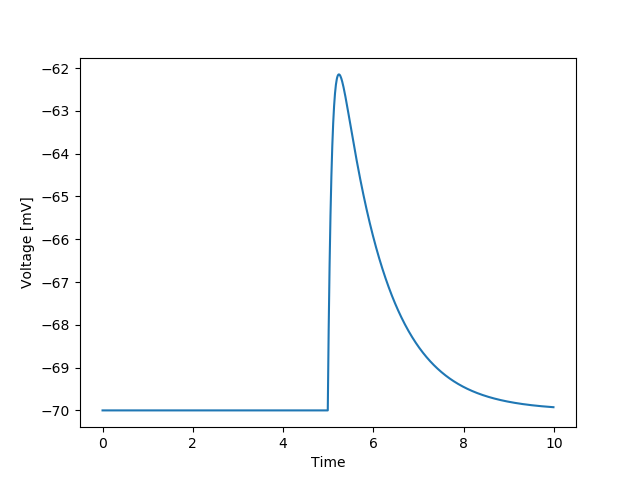
\includegraphics{c.png}
\end{itemize}
\end{document}
